\section{Motivation}
\begin{frame}{Main Problem: Sample Inefficiency}
\begin{itemize}
    \item Number of times the agent must interact with the environment in order to learn a task
    \vspace{0.5em}
    \item Good sample complexity is the first prerequisite for successful skill acquisition.
    \vspace{0.5em}
    \item Learning skills in the real world can take a substantial amount of time
    \begin{itemize}
        \item can get damaged through trial and error
    \end{itemize}
\end{itemize}
\end{frame}
\begin{frame}{Main Problem: Sample Inefficiency}
\begin{itemize}
    \item ``Learning Hand-Eye Coordination for Robotic Grasping with Deep Learning and Large-Scale Data Collection'', Levine et al., 2016 \rref{8}
    \begin{itemize}
        \item 14 robot arms learning to grasp in parallel
        \item objects started being picked up at around 20{,}000 grasps
    \end{itemize}
\end{itemize}
\begin{figure}
    \centering
    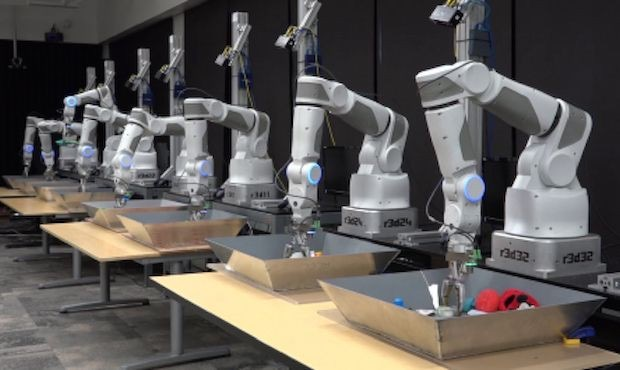
\includegraphics[width=0.6\textwidth,height=0.55\textheight,keepaspectratio]{images/soft-actor-critic/figures/robot-grasping-farm.jpg}
\end{figure}
\begin{flushright}
    \tiny\url{https://spectrum.ieee.org/automaton/robotics/artificial-intelligence/google-large-scale-robotic-grasping-project}
\end{flushright}
\end{frame}
\begin{frame}{Main Problem: Sample Inefficiency}
\begin{columns}[T]
\begin{column}{0.5\textwidth}
\vspace{1em}
\emph{Observing the behavior of the robot after over 800{,}000 grasp attempts, which is equivalent to about 3000 robot-hours of practice, we can see the beginnings of intelligent reactive behaviors.}
\end{column}
\begin{column}{0.5\textwidth}
\begin{figure}
    \centering
    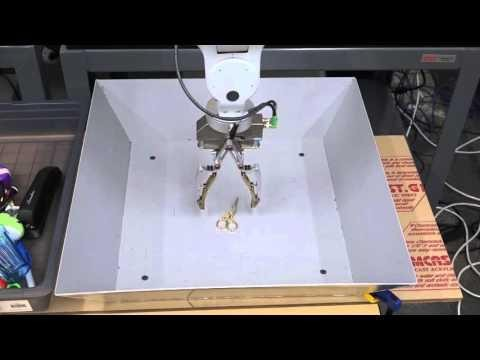
\includegraphics[width=\linewidth,height=0.6\textheight,keepaspectratio]{images/soft-actor-critic/figures/robot-grasping.jpg}
\end{figure}
\end{column}
\end{columns}
\begin{flushright}
    \tiny\url{https://www.youtube.com/watch?v=cXaic_k80uM}
\end{flushright}
\end{frame}
% (Near-blank "Solution? Off-Policy!" frame removed in Day 6 review --
%  the point is folded into the On-Policy vs Off-Policy recap in background.tex.)
